\newpage
\clearpage
\pagenumbering{arabic}
\setcounter{page}{13}

\section{Introdução}
\label{intro:intro}

A segmentação de imagens tem sido de extrema importância em meio ao contexto de visão computacional e entendimento de cenas, assim como uma grande auxiliadora para as questões relacionadas a atividades humanas. É visível que as segmentações sozinhas não causam um efeito de ação, mas são amplamente utilizadas como forma de auxiliar atividades humanas, das quais se destaca as análises das áreas médicas \citep{Lai2015, Withey2008} e exemplifica-se por meio da extração de limite de tumor \citep{Malkanthi2017}, medição de volumes de tecido e mapeamento de órgãos específicos em exames de imagem \citep{Gibson2018, Schoppe2020}, como é possível observar na Figura \ref{intro:fig:1}.

\begin{figure}[H]
    \centering
    \caption{Exemplos de segmentação no contexto médico. Representação de segmentação de vasos sanguíneos, câncer de pele, câncer pulmonar e núcleos celulares, respectivamente.}
    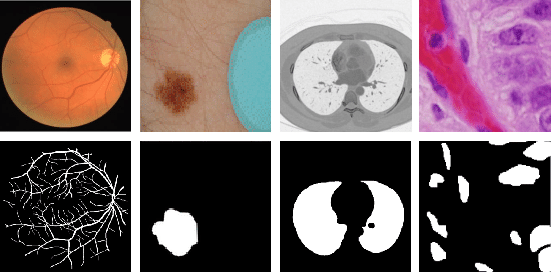
\includegraphics[width=1\linewidth]{recursos/imagens/introduction/medical-image-segmentation.png}
    \label{intro:fig:1}

    Fonte: \cite{Asadi-Aghbolaghi2020}.
\end{figure}

Outro contexto que tem usufruído muito das segmentações, que são aplicadas em imagens e vídeos, é o de sistemas autônomos \citep{Kaymak2019, Liu2020, Pan2020, Teichmann2018}, dos quais se cita os de máquinas empresariais para controle de qualidade e os carros autônomos, que necessitam realizar a segmentação de pedestres, placas e sinaleiros, como nos trabalhos realizados por \cite{Lee2018, Fleyeh2004} e \cite{Pan2020}, dos quais é possível observar exemplos a partir da Figura \ref{intro:fig:2}.

\begin{figure}[H]
    \centering
    \caption{Exemplos de segmentação feita por sistemas autônomos.}
    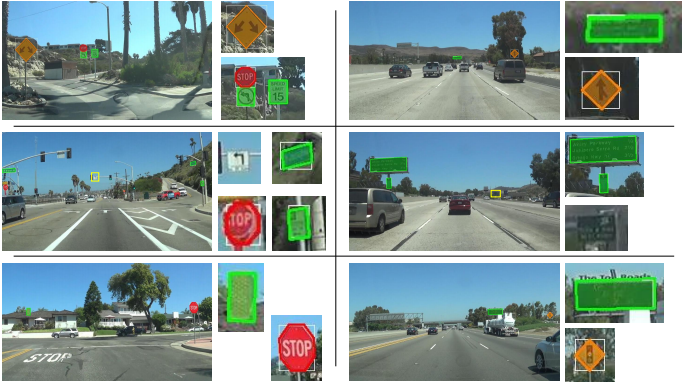
\includegraphics[width=1\linewidth]{recursos/imagens/introduction/placas.png}
    \label{intro:fig:2}

    Fonte: \cite{Lee2018}.
\end{figure}

Todavia, como citado no início deste capítulo, as segmentações não geram diretamente uma ação, mas são altamente difundidas como um processo intermediário para o reconhecimento de imagens ou detecção de objetos, como ocorre no trabalho executado por \cite{Carneiro2021}, que utiliza do método \textit{GrabCut} \citep{rother2004grabcut}, um método de segmentação baseado em grafos (que também são comuns no contexto de segmentação, como apresentado por \cite{Yi2012}) para realizar a segmentação das folhas de café antes de realizar a detecção de doenças e pragas na folha do café, como demonstrado na Figura \ref{intro:fig:3}. Este tipo de abordagem para as segmentações de imagens é muito comum como forma auxiliar em relação ao fluxo completo de sistemas de visão computacional.

\begin{figure}[H]
    \centering
    \caption{Segmentação feita com \textit{GrabCut}.}
    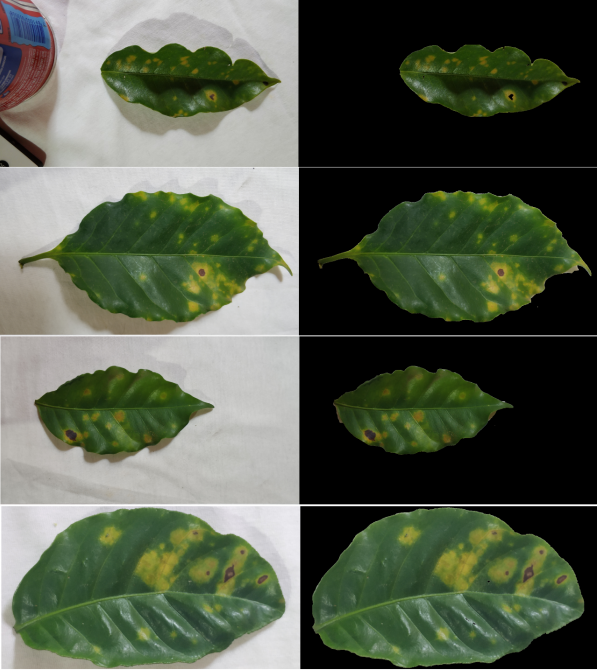
\includegraphics[height=3in]{recursos/imagens/introduction/grabcut.png}

    \label{intro:fig:3}

    Fonte: \cite{Carneiro2021}.
\end{figure}

Quanto às áreas de aplicação que viabilizam o uso das técnicas de segmentação e podem usufruir da mesma, vale citar também a área odontológica, em que há uma busca em relação à exploração de todos os componentes presentes na boca dos pacientes, desde doenças (como as cáries) até a contagem e classificação de saúde dos dentes. Para várias dessas atividades, o diagnóstico é acompanhado de análises de imagens clínicas, buscando evidenciar as necessidades com o uso de aparelhos \citep{Schwendicke2020}. Deste modo, como citado por \cite{Bansal2021, Nguyen2021} e \cite{Schwendicke2020}, destaca-se que as soluções para esses tipos de problemas têm sido encontradas com a aplicação de inteligência artificial que aumentam o desempenho da atuação humana. A Figura \ref{intro:fig:4} exemplifica algumas aplicações desenvolvidas com o intuito de segmentar dentes e cáries.

\begin{figure}[H]
    \centering
    \caption{Exemplo de segmentação na área odontológica.}
    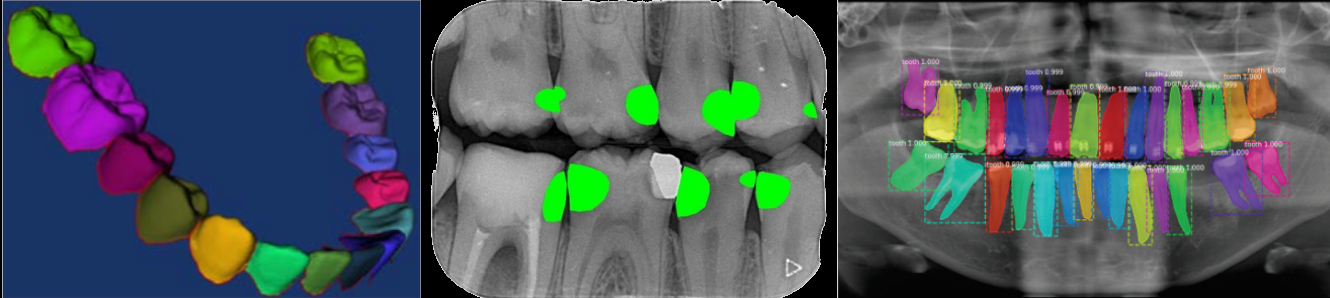
\includegraphics[width=1\linewidth]{recursos/imagens/introduction/odonto_segmentation.png}
    \label{intro:fig:4}

    Fonte: retirado e adaptado de \cite{Shuai2016,Bayrakdar2021,Gil2019}, respectivamente.
\end{figure}

Dentre as abordagens de segmentação, vale dizer que muitos algoritmos foram desenvolvidos para suprir a necessidade de segmentação, dos quais se destacam métodos artesanais (que serão trabalhados no Capitulo \ref{segment:image}), como os baseados em região ou limiar (Seção \ref{segment:region}), em bordas (Seção \ref{segment:limit}) e agrupamentos (Seção \ref{segment:group}) ou até em métodos mais complexos, devido ao progresso proporcionado pelos avanços de redes neurais, como os algoritmos baseados nessa hipótese (Seção \ref{segment:neural}).

Na medida em que algumas propostas utilizadas em inteligência artificial vêm avançando, observa-se diversos avanços nas áreas de aprendizado profundo, tendo grande destaque e evolução quanto ao âmbito de segmentação de imagens. Esses avanços ocorrem não só devido a um \textit{hardware} com mais capacidade de processamento ou uma maior quantidade de dados disponíveis, mas também por causa da criação de novos algoritmos e abordagens para resolver esses problemas \citep{Szegedy2015}.

A partir desses modelos mais modernos que utilizam como recurso o aprendizado profundo, cita-se que estes possuem capacidade de segmentar e propor classes para todos os pixels de uma imagem \citep{Minaee2021}, outros são capazes de segmentar objetos de mesma classe como instâncias diferentes, ou ainda outros que propõe fazer a unificação de ambas propostas anteriores dando um maior detalhamento das cenas, como é o caso das segmentações semânticas (Capitulo \ref{semantic:semantic}), de instâncias (Capitulo \ref{instance:instance}) e panóptica (Capitulo \ref{panoptic:panoptic}), respectivamente.

Com o avanço das técnicas de segmentação mais modernas, tornou-se possível trabalhar com um maior volume de dados presentes nas imagens, abrindo oportunidades para a realização de experimentos relacionados à escala dos objetos presentes na cena e à dimensionalidade preservada pelos modelos. No entanto, mesmo com as abordagens de segmentação mais avançadas, a segmentação de objetos pequenos na imagem ainda representa um grande desafio \citep{Sang2023Small-ObjectAttention, Su2021Small-scaleFusion}.

O tratamento de objetos em pequena escala oferece perspectivas promissoras para aplicações na área odontológica, entre outras. Compartilhando diversos desafios específicos, a área odontológica pode se beneficiar da aplicação de modelos modernos de segmentação, como demonstrado por \cite{Ghazvinian2021} e \cite{Minyoung2020}, em contraste com a prática mais comum de utilizar métodos tradicionais \citep{Hammad2020}. O desenvolvimento de projetos de segmentação voltados para essa área pode auxiliar profissionais a descreverem a saúde bucal do paciente, contribuindo significativamente para o diagnóstico \citep{Ghazvinian2021}.

No presente projeto serão listados alguns modelos de algoritmos e \textit{frameworks} conhecidos, dos quais alguns são definidos como estado-da-arte (\textit{Mask} R-CNN e U-Net, por exemplo), de modo que estes estejam relacionados a segmentações e que seja possível encontrar vantagens, desvantagens e possibilidades de exploração em relação aos mesmos para basear novos experimentos, assim, contribuindo para a evolução científica na esfera de segmentações, principalmente das que fazem uso de aprendizado profundo.

Assim, espera-se que esta investigação possa contribuir para a geração futura de uma ferramenta automática para a geração detalhada de sobre as condições bucais e dentais de pacientes. Além de poder contribuir com os profissionais dentistas, isso pode contribuir como uma ferramenta de auxílio inicial ao diagnóstico e triagem, algo importante para locais do planeta que possuem recursos e acessos escassos para o tratamento odontológico.


\section{Block-based Principal Component Analysis Pooling (BPCA Pooling)}
\label{intro:bpca}
Apresentado como uma variação do método convencional do Principal Component Analysis (PCA) no trabalho \cite{Salvadeo2011}, o BPCA propõe um método que inicialmente foi utilizado para a extração de características de imagens relacionadas a trabalhos de reconhecimento de face, propondo um método de extração que trouxesse à análise menor custo computacional, redução de dimensionalidade e uma geometria de hiperespaço que fosse mais intuitiva, destacando o diferencial de que com esse método fosse possível preservar a espacialidade da informação.

O método proposto opera por meio da subdivisão de uma imagem em blocos $k \times k$, em que os blocos geralmente possuem tamanhos iguais (por exemplo, $3 \times 3$, $8 \times 8$, etc.). Em seguida, o PCA é aplicado a cada um desses blocos subdivididos. Consequentemente, cada bloco $k \times k$ passa a ter um tamanho reduzido, contendo apenas um subconjunto de pixels com $r$ características (o mesmo numero de blocos). Esse processo pode ser visualizado através da Figura X.

É importante ressaltar que o BPCA não é uma simples combinação linear de amostras distintas. Em vez disso, ele cria uma representação organizada, formada por pequenos blocos do mapa de características original usado como entrada. O BPCA incorpora o PCA para realizar o mapeamento não supervisionado que minimiza o erro quadrático médio entre a entrada original e a representação projetada.

Considerando os parágrafos anteriores e o fato de que as camadas de pooling são aplicadas com sucesso nas redes convolucionais com o objetivo de reduzir a dimensionalidade dos dados \cite{paul2019dimensionality}, a partir do presente trabalho, propõe-se a utilização dessa técnica não para a tarefa de extração de características, mas como uma camada de pooling que contenha o benefício de preservar a espacialidade da informação entre as camadas convolucionais.

A camada de pooling adota o processo original do BPCA, que extrai as principais informações de cada bloco, reduzindo a dimensionalidade dos dados e preservando características relevantes. Além disso, o método foi aprimorado por meio da normalização dos blocos usando média ($\mu$) e desvio padrão ($\sigma$). Em seguida, é aplicada a decomposição em valores singulares (SVD) para extrair os componentes principais ($\text{{pca\_components}}$) que realizam a transformação dos blocos por meio da projeção nesses componentes selecionados. Como resultado, obtém-se um mapa de características reduzido em tamanho, mas que preserva a informação essencial ao concatenar os blocos transformados.

A representação matemática do processo realizado pela camada de pooling BPCAPooling pode ser descrita pela seguinte equação:

\[
\text{{BPCAPooling}}(x) = \text{{reshape}}\left(\text{{SVD}}\left(\frac{{x - \mu}}{{\sigma}}\right) \cdot \text{{pca\_components}}\right),
\]
onde $x$ representa o mapa de características de entrada, $\text{{reshape}}$ reorganiza os blocos transformados em uma estrutura de saída adequada, $\text{{SVD}}$ denota a decomposição em valores singulares dos blocos normalizados, $\mu$ é o vetor médio dos blocos extraídos, $\sigma$ é o vetor de desvio padrão dos blocos extraídos, e $\text{{pca\_components}}$ é uma matriz que contém os primeiros componentes principais selecionados.

Essa formulação matemática descreve o processo de pooling realizado pela camada BPCAPooling, que extrai informações relevantes dos blocos de entrada, reduzindo sua dimensionalidade e preservando características importantes para o aprendizado eficiente da rede neural convolucional.


\subsection{Objetivos}
\label{intro:objective}

\subsection{Considerações Finais do Capítulo}
\label{intro:end}

Por fim, nos capítulos seguintes, assuntos relacionados à apresentação de conceitos de redes neurais profundas e redes neurais convolucionais serão tratadas no Capítulo \ref{deep:deep}. Após, será discorrido sobre as técnicas que tradicionalmente são utilizadas para atividades de segmentação no Capítulo \ref{segment:image}, acompanhada de segmentações que são fruto do advento das redes convolucionais e aprendizado profundo, tratando da segmentação semântica (Capítulo \ref{semantic:semantic}), de instâncias (Capítulo \ref{instance:instance}) e panóptica (Capítulo \ref{panoptic:panoptic}), para quê, finalmente sejam apresentados os detalhes da metodologia proposta nesse trabalho de forma clara no Capítulo \ref{proposal:proposal}.  Finalmente, o Capítulo \ref{final:final} apresenta algumas considerações finais do trabalho.